%\documentclass[compress]{beamer}

\documentclass[12pt]{beamer}
\usepackage{etex}
\usetheme{CambridgeUS}
\setbeamertemplate{headline}{}
\usecolortheme{seahorse}
\definecolor{UniBlue}{RGB}{83,121,170}
\setbeamercolor{frametitle}{fg=UniBlue}
\setbeamertemplate{navigation symbols}{}
%\setbeamercolor{itemize item}{fg=red}
%\beamertemplatenavigationsymbolsempty
%\setbeamertemplate{navigation symbols}{}
%\useoutertheme{default}

\usepackage{makeidx}  % allows for indexgeneration
\usepackage{mathtools} %
\usepackage{booktabs} %
\usepackage{verbatim} %
\usepackage{graphicx} %
\usepackage[labelformat=empty]{caption}
\usepackage{amsmath}
\usepackage{amssymb}
\usepackage{amsthm}
\usepackage{xspace}
\usepackage{multirow}
\usepackage{subfig}
\usepackage{pifont}
\usepackage{empheq}
\usepackage{relsize}
\usepackage{slashbox}
\usepackage{textcomp}
\usepackage{picture}
\usepackage{float}
\usepackage{url}
\usepackage{tikz}

%\usepackage[latin1]{inputenc}
%\usefonttheme{professionalfonts}
%\usepackage{times}
%\usetikzlibrary{arrows,shapes}

\usepackage[T1]{fontenc}
\usepackage{algorithmic} 
\usepackage{xparse}
%\usepackage[backend=bibtex,style=authortitle]{biblatex}
\usepackage[backend=bibtex,style=authortitle-ibid]{biblatex}
%\usepackage[backend=bibtex,style=mla]{biblatex} 
\addbibresource{present-bibli.bib}
\renewcommand{\footnotesize}{\tiny}
% \usepackage{algpseudocode} 
%\usepackage{algorithm}
%\usepackage[vlined]{algorithm2e} 

\usetikzlibrary{calc}

% tikzmark command, for shading over items
\newcommand{\tikzmark}[1]{\tikz[overlay,remember picture] \node (#1) {};}


\makeatletter
% \cvhrulefill{<color>}{<thickness>}
\newcommand*\cvhrulefill[2]{%
  \leavevmode\color{#1}\leaders\hrule\@height#2\hfill \kern\z@\normalcolor}
% \crule{<color>}{<width>}{<thickness>}
\newcommand*\crule[3]{%
  \color{#1}\rule{#2}{#3}\normalcolor}
\makeatother

\author{{\normalsize Emre Sefer \and Geet Duggal}
  \\ 
\vspace{0.65cm}
%{Carnegie Mellon University} \\
\vspace{1.75cm}

\includegraphics[width=2.0cm]{cmulogo.jpeg} \hspace{5cm} 
\includegraphics[width=1.5cm]{cpcblogo.jpeg}}

\title{{\bf \Large Hi-C Tutorial: Topological Domains }}

\normalsize

\newcommand{\Armatus}{\emph{Armatus}\xspace}


\makeatletter
\def\overUnderArrow{\@ifnextchar[\overUnderArrow@i{\overUnderArrow@i[]}}
\def\overUnderArrow@i[#1]#2#3{% #1 under #2 over #3 main argument
  \ifx\relax#1\relax\array[b]{c}\overset{\text{#2}}{\uparrow}\\#3\endarray
  \else\ifx\relax#2\relax
    \array[t]{c}#3\\\underset{\text{#1}}{\downarrow}\endarray
  \else
    \array{c}\overset{\text{#2}}{\uparrow}\\#3\\\underset{\text{#1}}{\downarrow}\endarray
  \fi\fi}
\makeatother

\definecolor{Green}{rgb}{0,0.5,0}

\newcommand*{\boxedcolor}{red}
\makeatletter
\renewcommand{\boxed}[1]{\textcolor{\boxedcolor}{%
  \fbox{\normalcolor\m@th$\displaystyle#1$}}}
\makeatother

\begin{document}

%\captionsetup[figure]{labelformat=empty}
\setbeamertemplate{footline}{} 
\date{}

{\usebackgroundtemplate{%
\tikz\node[opacity=0.2]{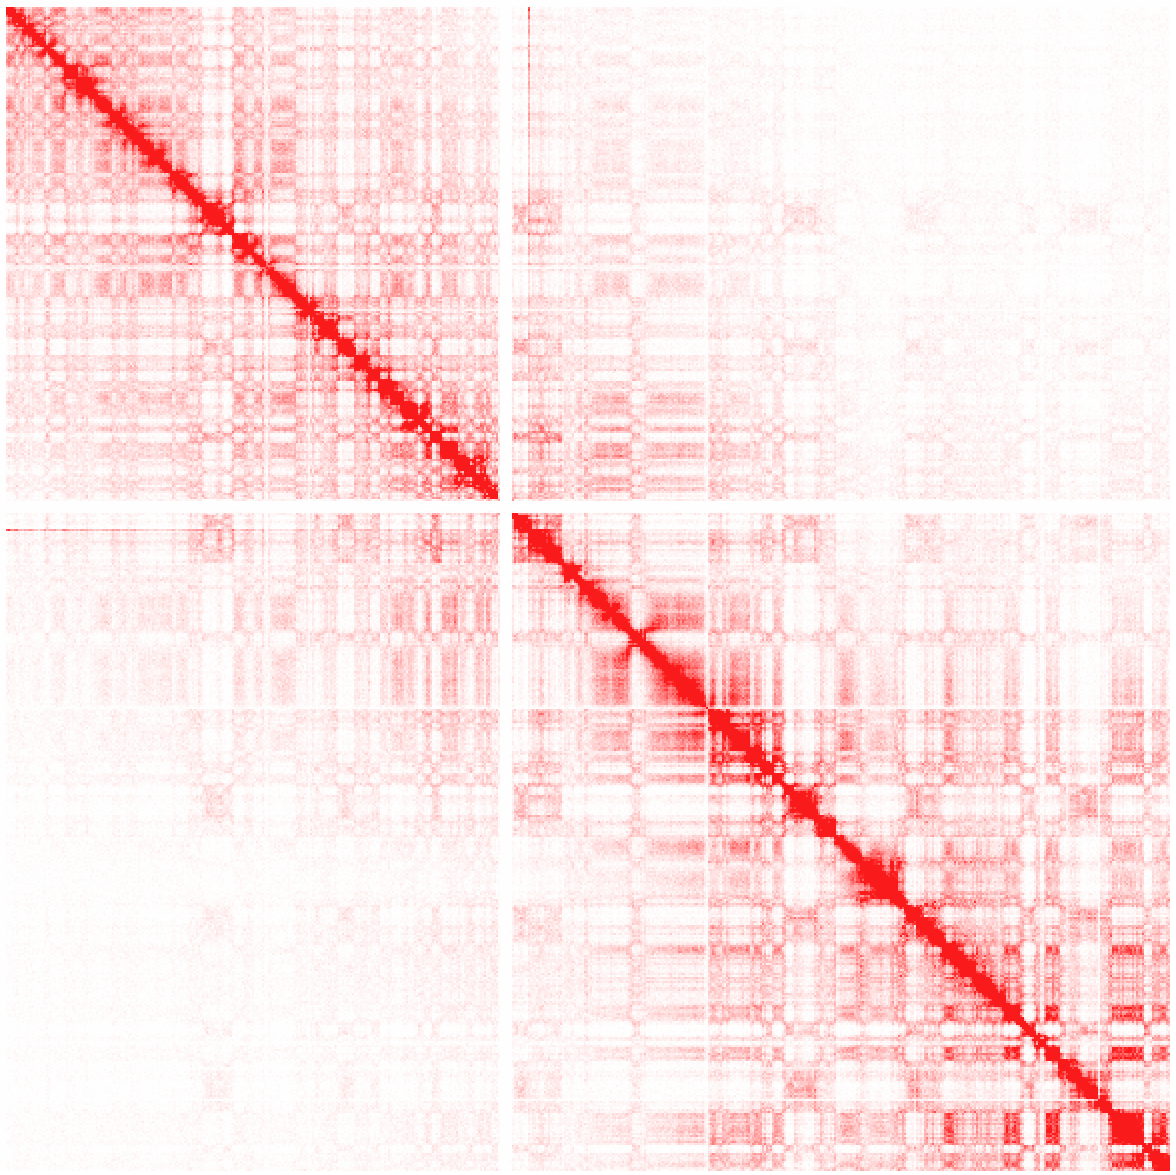
\includegraphics[height=0.9\paperheight,width=0.9\paperwidth]{hicpic2.png}};}
\frame{\titlepage}}


\begin{frame}
\frametitle{What is a Topological Domain?}


\end{frame}


\begin{frame}
\frametitle{What is a Topological Domain?}


\end{frame}


\begin{frame}
\frametitle{Chromatin Hierarchy}


\end{frame}


\begin{frame}
\frametitle{Chromatin Classification by PCA}

%\begin{figure}
%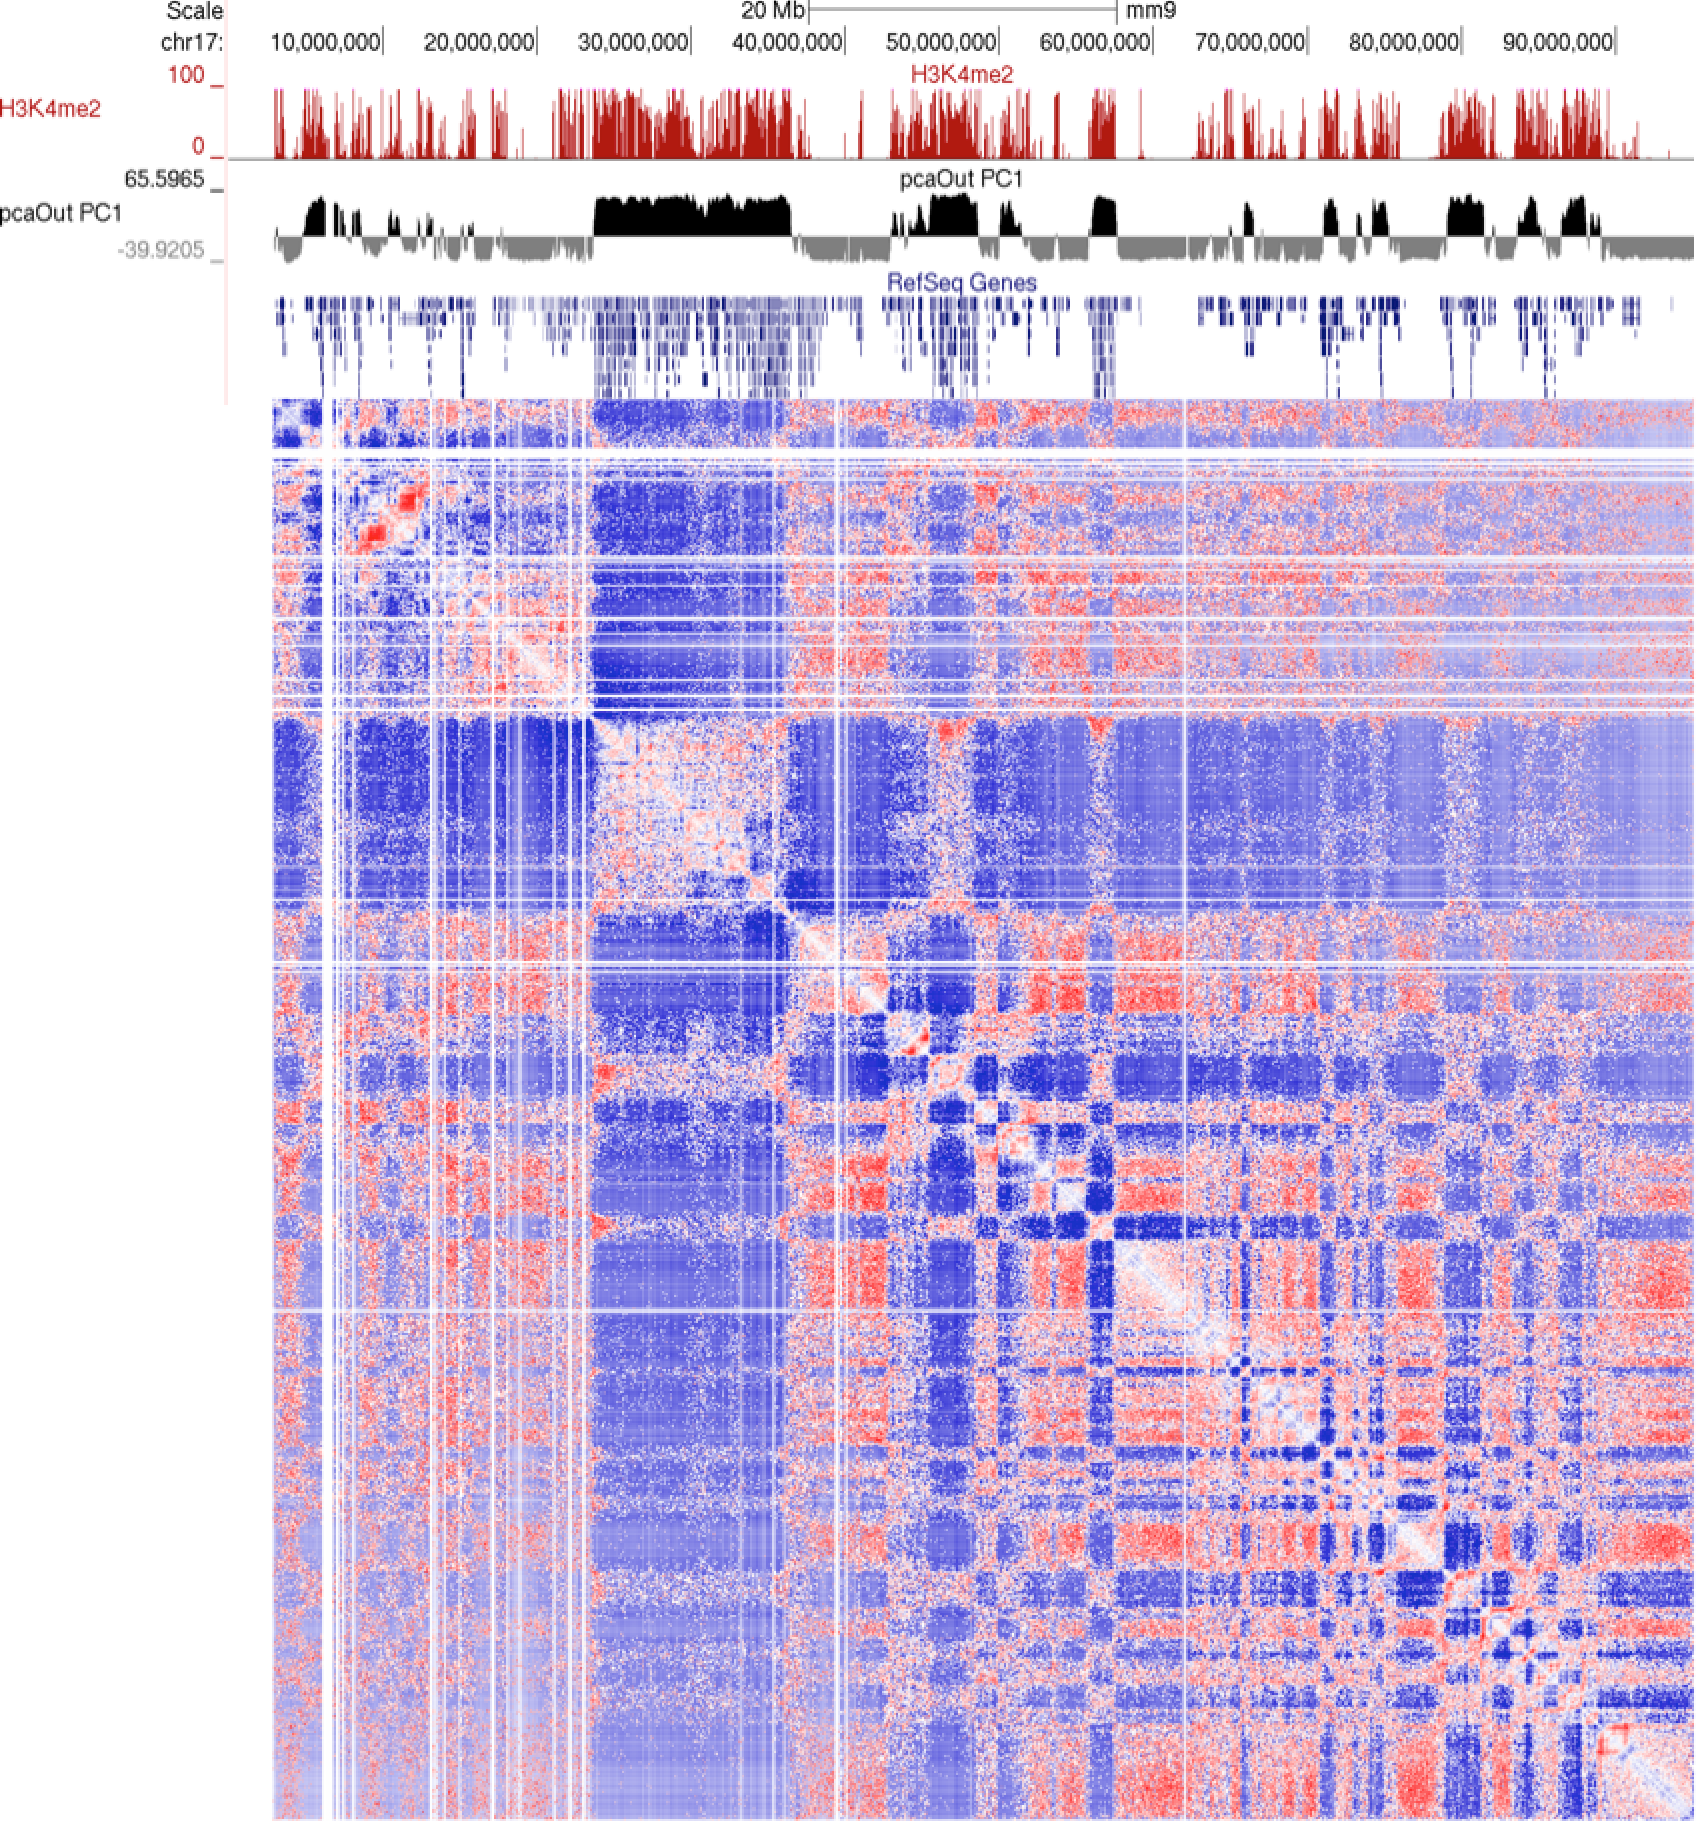
\includegraphics[scale=0.07]{pcamatrix.png}
%\end{figure}
\begin{figure}
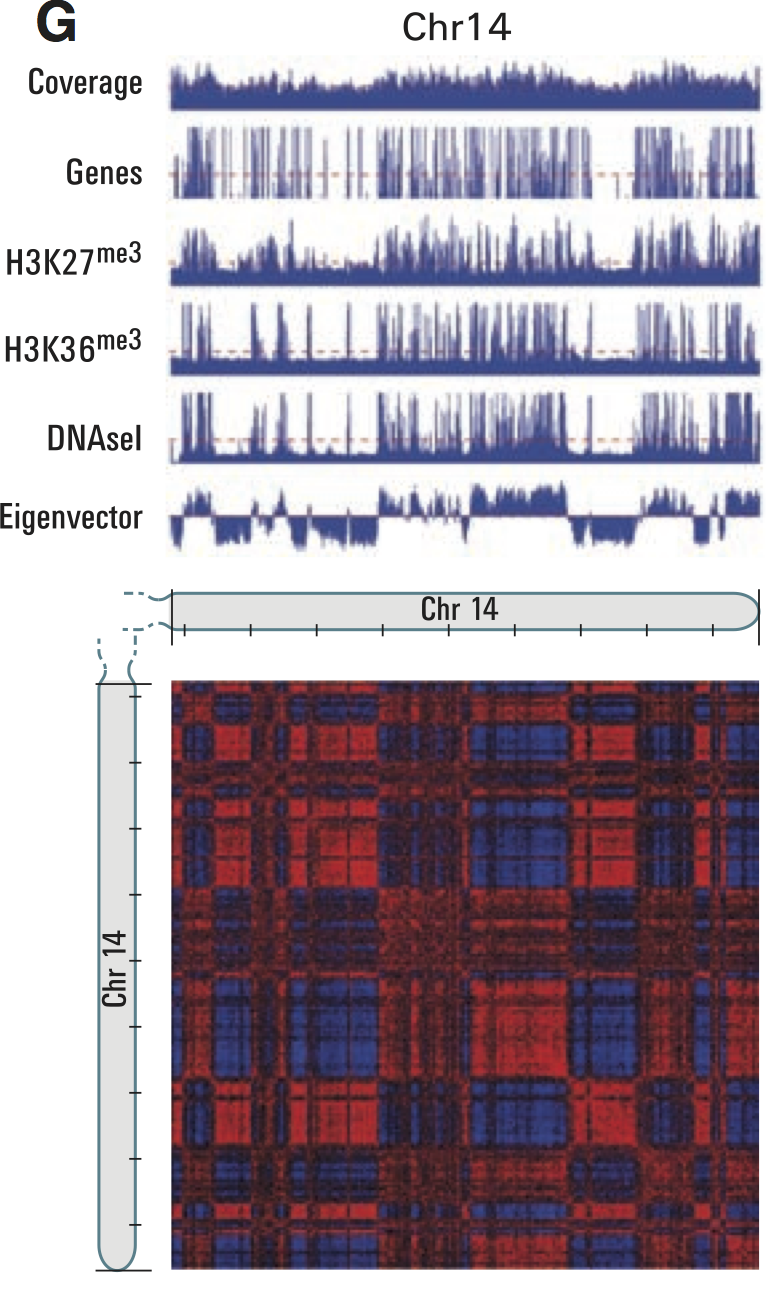
\includegraphics[scale=0.46]{eigen.png}
\end{figure}

%Classification of genomic domains with respect to gene activity, function, and nuclear
%compartments
\begin{itemize}
\item Human chromosomes are partitioned into two types of
  compartments:
\begin{itemize}
\item Compartment A -> open chromatin -> active gene-dense regions 
\vspace{0.07cm}
\item Compartment B -> closed chromatin -> repressive gene-poor regions
\end{itemize}
\end{itemize}

\footcitetext{aiden}

\end{frame}


\begin{frame}
\frametitle{TADs Are Enriched For Genomic Features}

\begin{figure}
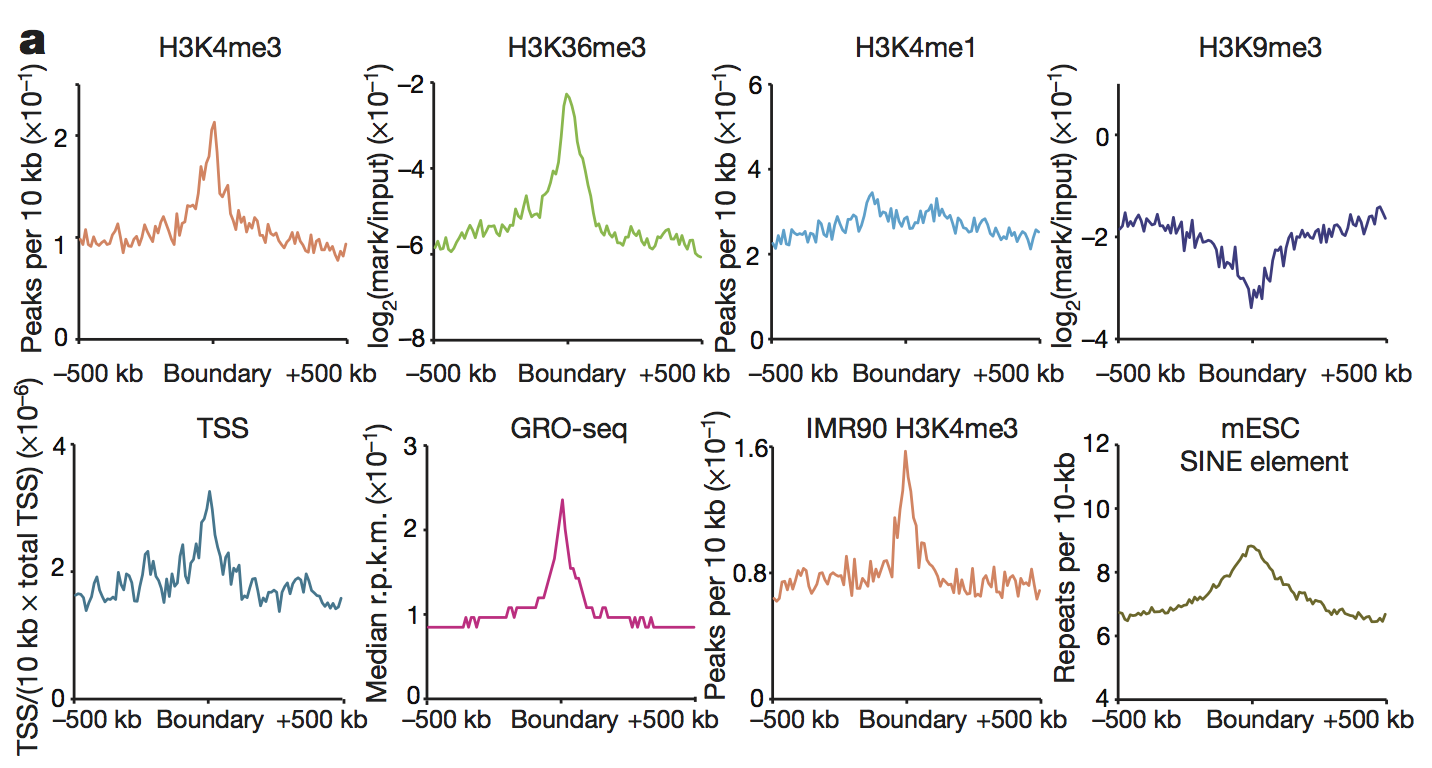
\includegraphics[scale=0.85]{feature.png}
\end{figure}

\begin{itemize}
\item H3k4me3 is enriched at TAD boundaries.
\vspace{0.1cm}
\item Repressive markers such as H3k9me3 are depleted at TAD boundaries.
\vspace{0.1cm}
\item CTCF binding sites are also enriched. 
\end{itemize}

\footcitetext{dixon2012}

\end{frame}


\begin{frame}
\frametitle{Domain Finder: Sexton et al.}

\begin{figure}
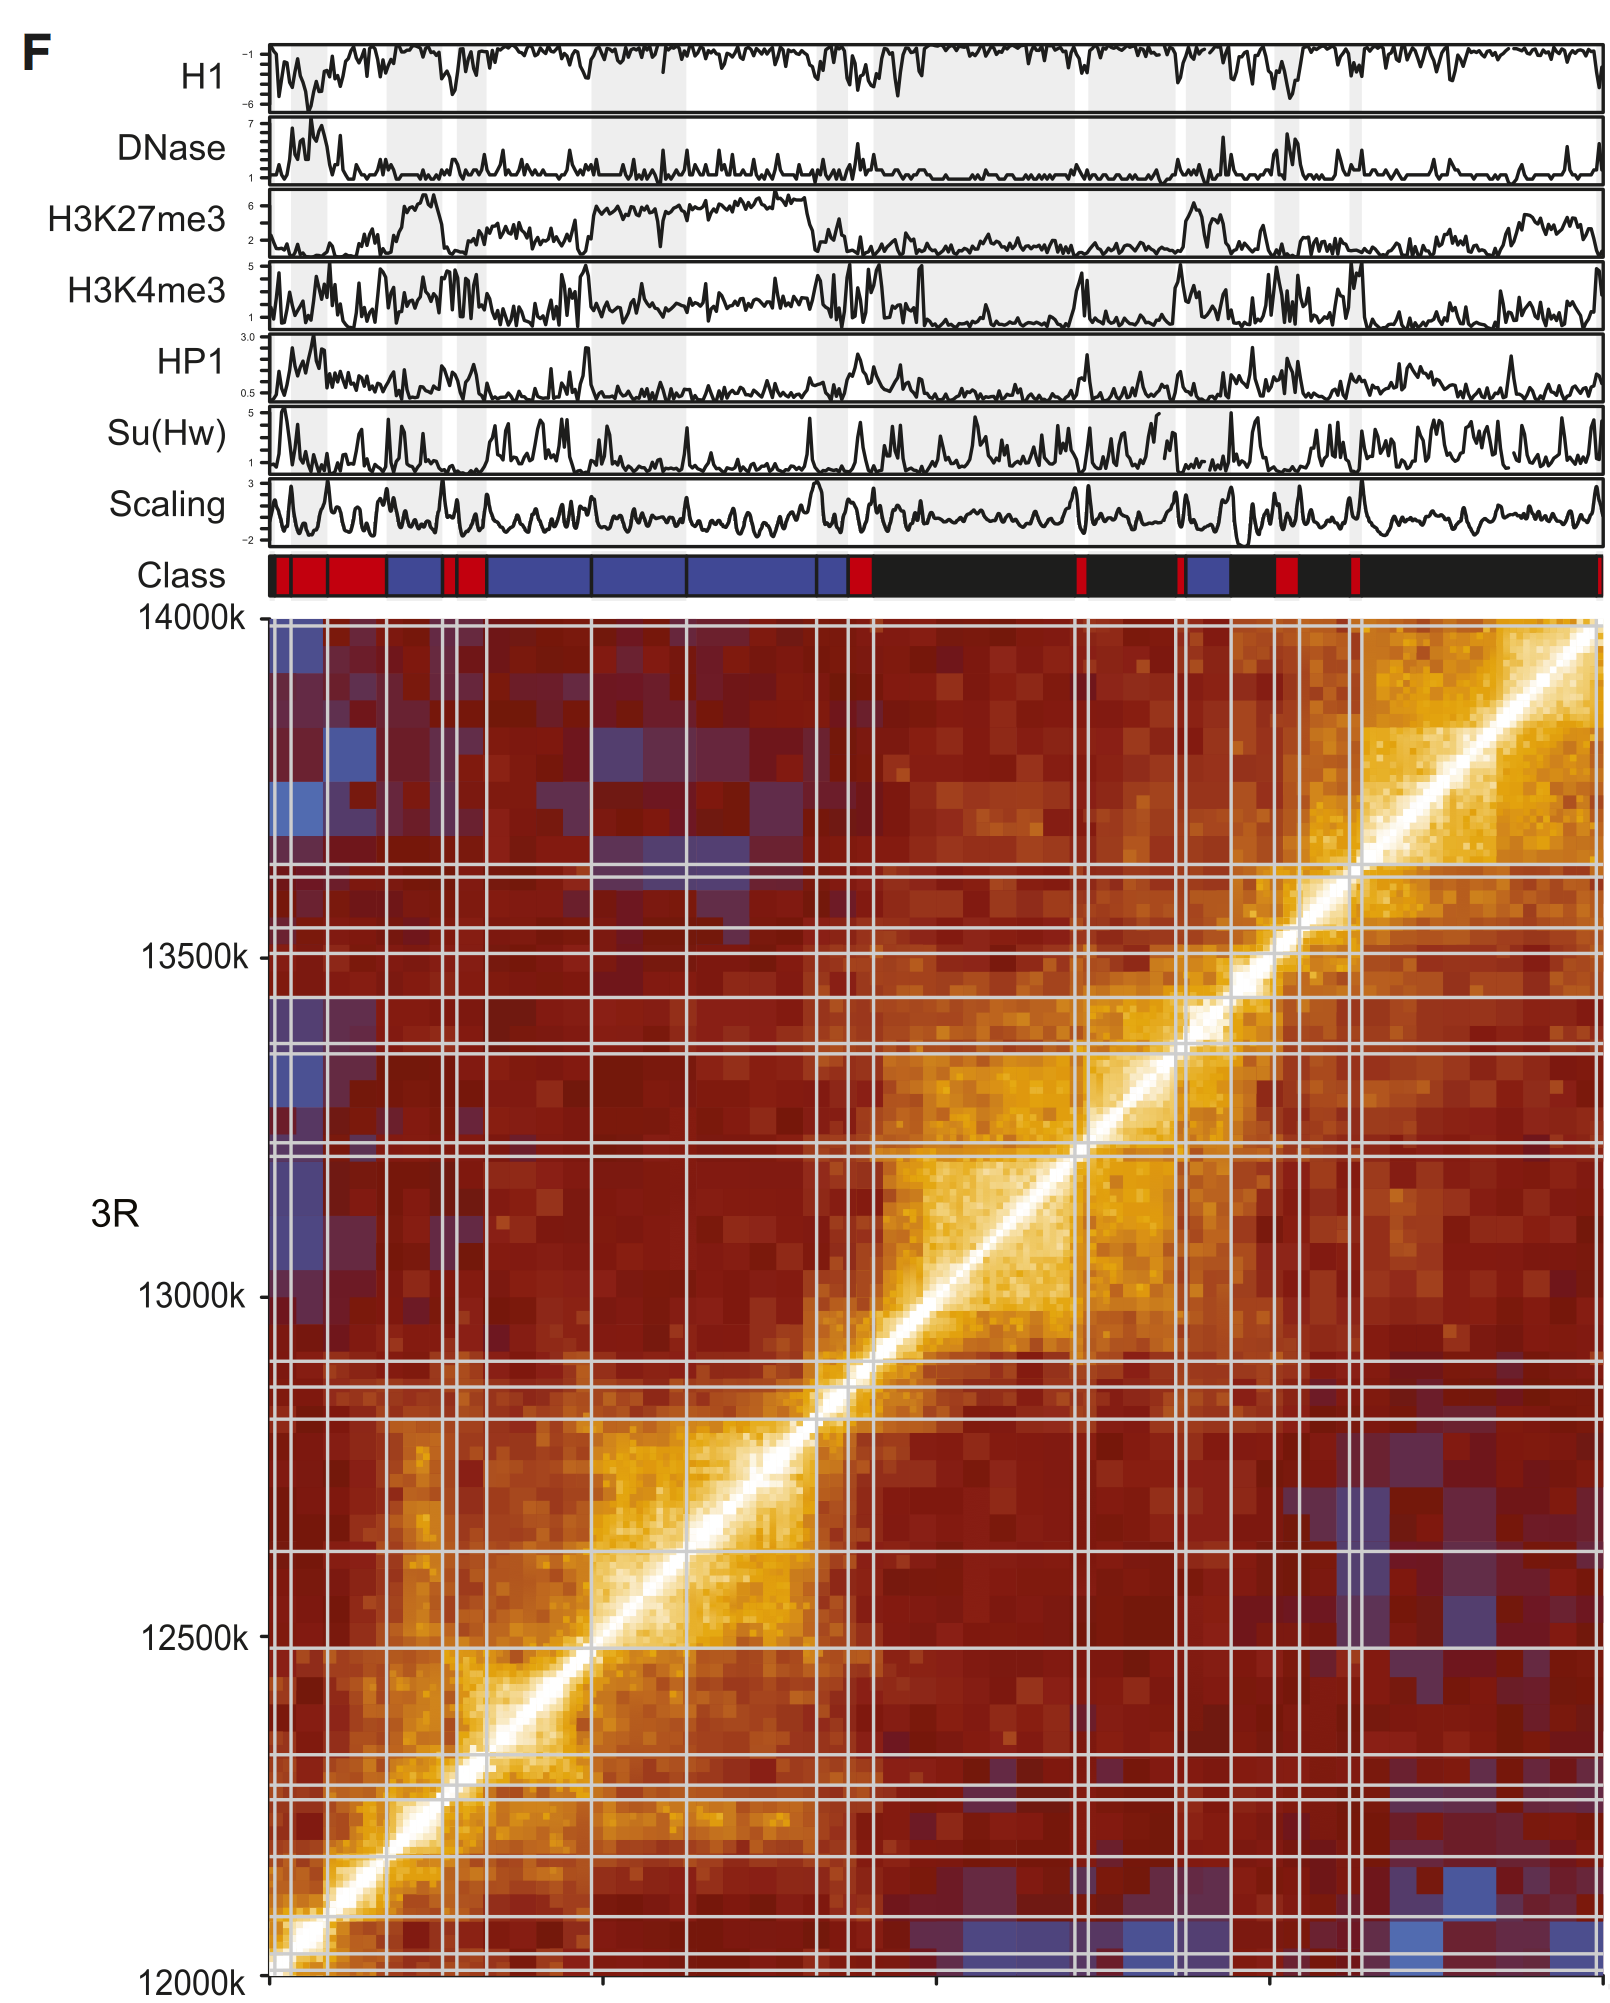
\includegraphics[scale=0.27]{dixon.png}
\end{figure}

\begin{itemize}
\item Domain partition based on likelihood optimization
\begin{figure}
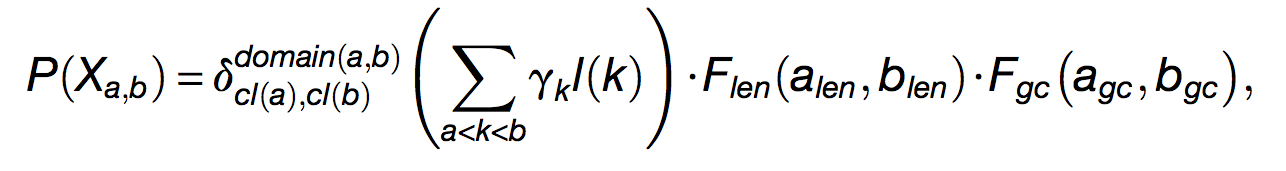
\includegraphics[scale=0.8]{dixoneq.png}
\end{figure}
\vspace{0.1cm}
\item TADs create unexpectedly low numbers of contacts crossing the
  boundary regions
\vspace{0.1cm}
\item Peaks correspond to domain boundaries
\end{itemize}

\footcitetext{sexton2012}

\end{frame}


\begin{frame}
\frametitle{Domain Finder: Arrowhead}

\begin{figure}
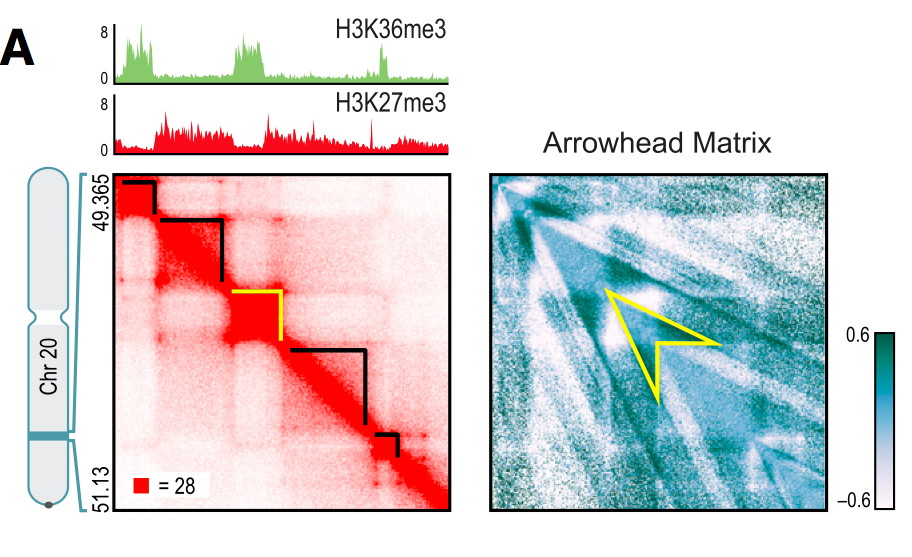
\includegraphics[scale=0.75]{arrowheadmatrix.png}
\end{figure}

\begin{itemize}
\item Builds modified difference matrix corresponding to
  directionality biases
\begin{itemize}
\item Search arrowhead pattern over this matrix heuristically
\end{itemize}
\vspace{0.1cm}
\item Find corners of domains by arrowhead search
\vspace{0.1cm}
\item Make use of very high resolution contact maps
\end{itemize}

\footcitetext{rao2014}

\end{frame}


\begin{frame}
\frametitle{Domain Finding via Deconvolution}

\begin{figure}
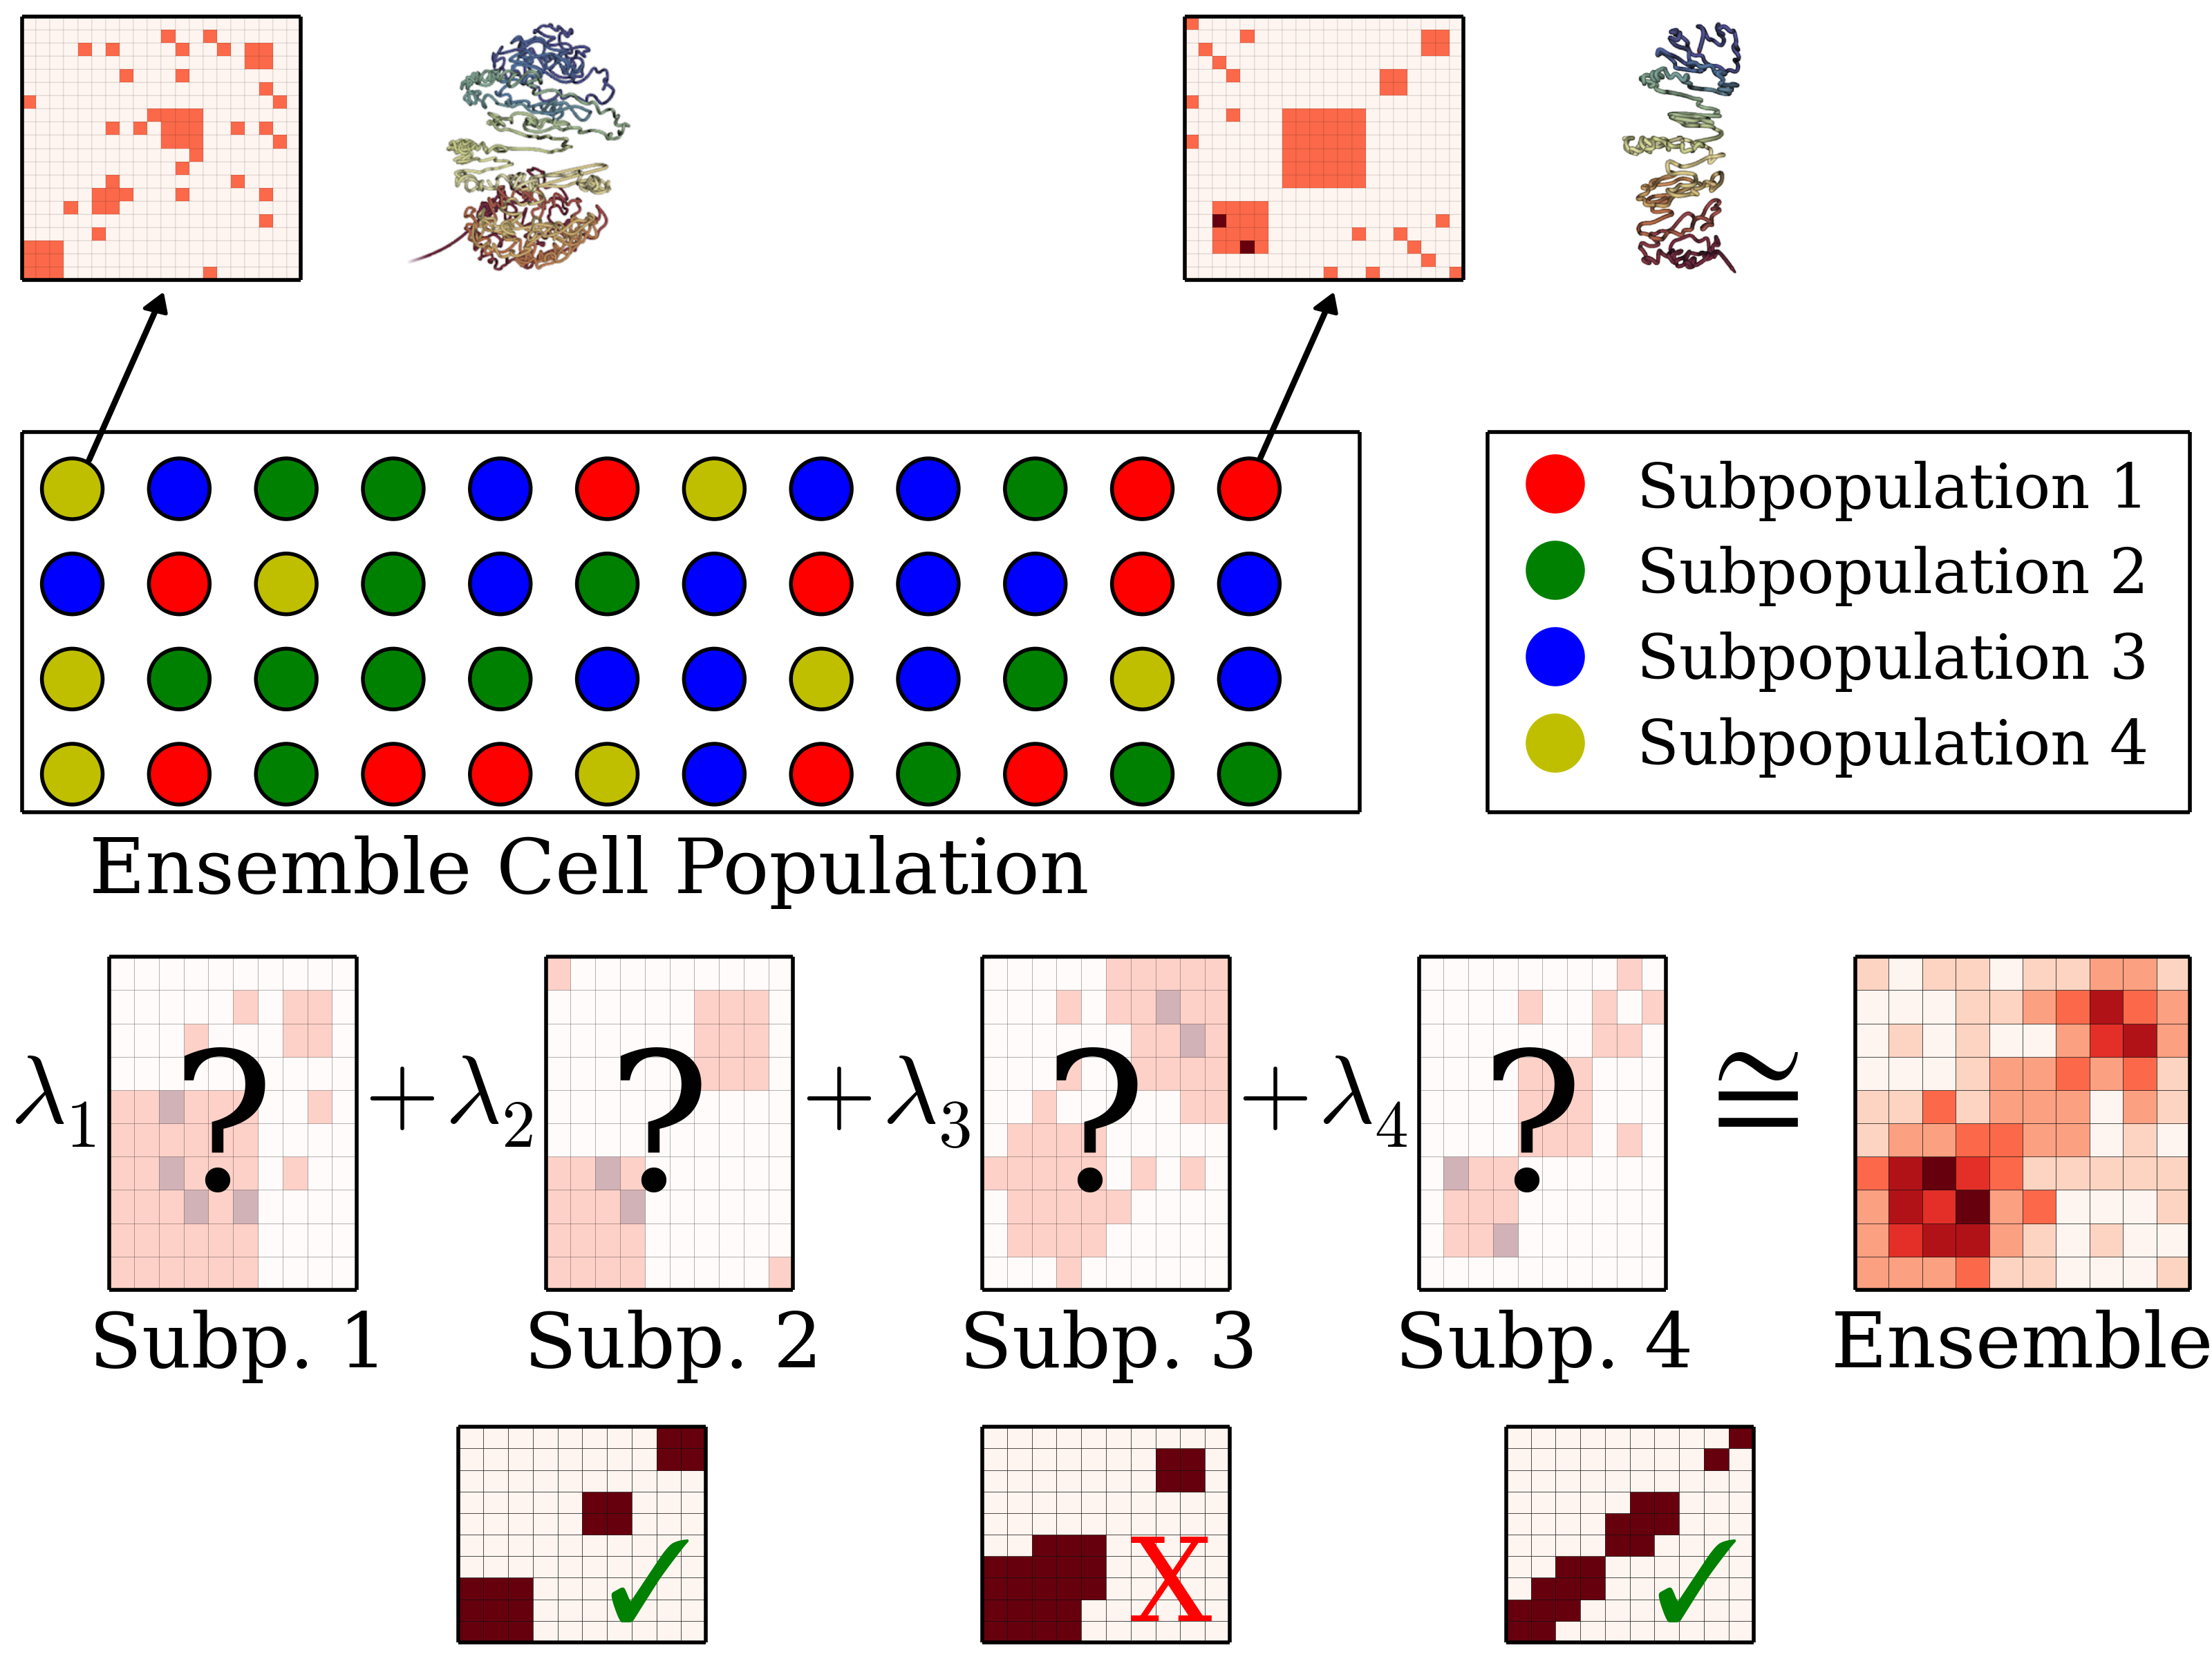
\includegraphics[scale=0.25]{decon_ex.png}
\end{figure}

\begin{itemize}
\item Deconvolution: Given an ensemble Hi-C matrix, can we extract the mixing
  components?
\begin{itemize}
\item Identify TADs indirectly by deconvolution
\vspace{0.05cm}
\item Domains in the context of structural classes
\end{itemize}
\vspace{0.1cm}
\item It is based on combinatorial optimization
\end{itemize}

\footcitetext{decon2015}

\end{frame}


\begin{frame}
\frametitle{Domain Finder: TADBIT}

\begin{figure}
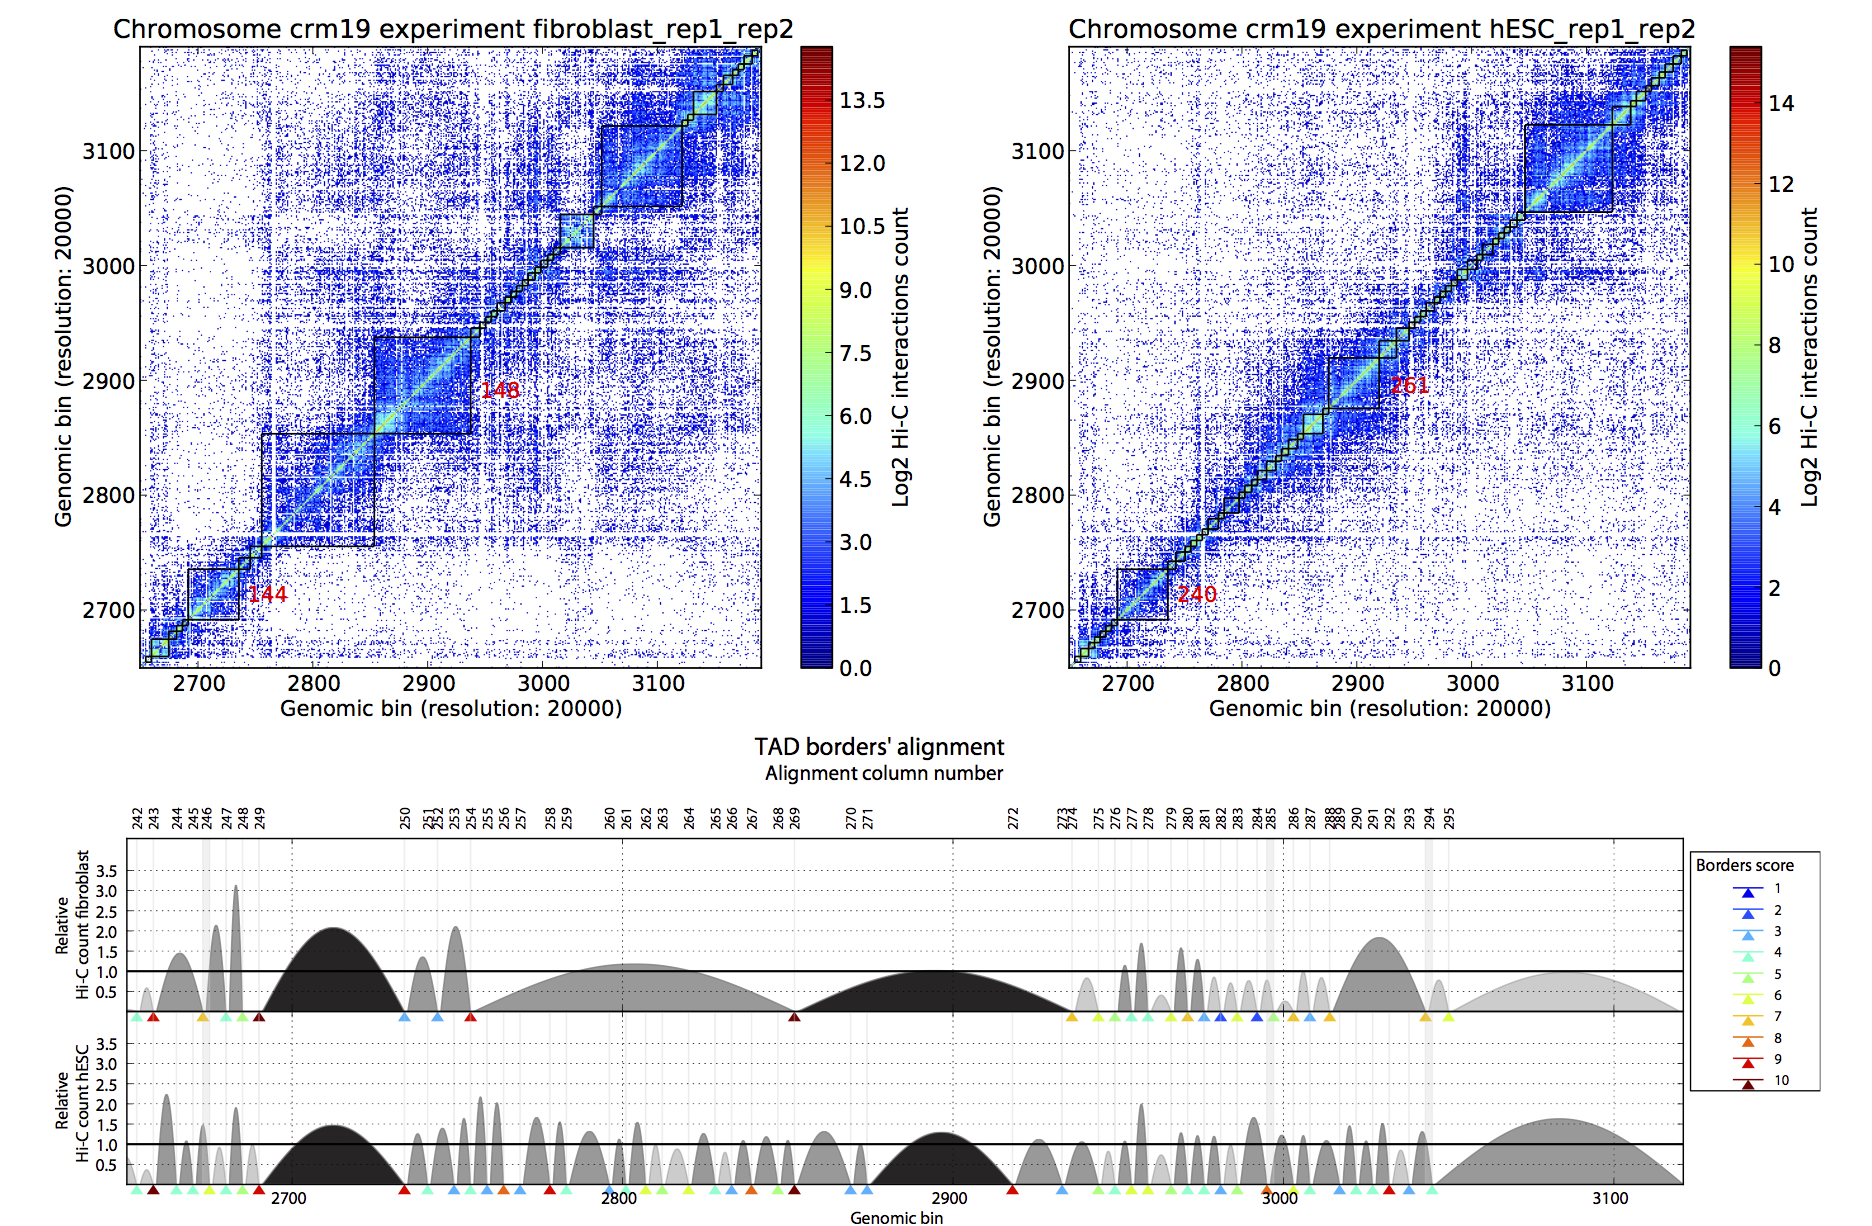
\includegraphics[scale=0.5]{tadbit.png}
\end{figure}

\begin{itemize}
\item TADBit uses breakpoint detection to detect TAD border positions
\begin{itemize}
\item It uses BIC penalized estimation of likelihood
\vspace{0.1cm}
\item Poisson assumption of Hi-C counts
\end{itemize}
\vspace{0.1cm}
\item Dynamic programming based algorithm
\end{itemize}

\footcitetext{tadbit}

\end{frame}


\begin{frame}
\frametitle{Domain Finder: HiCseq}

\begin{figure}
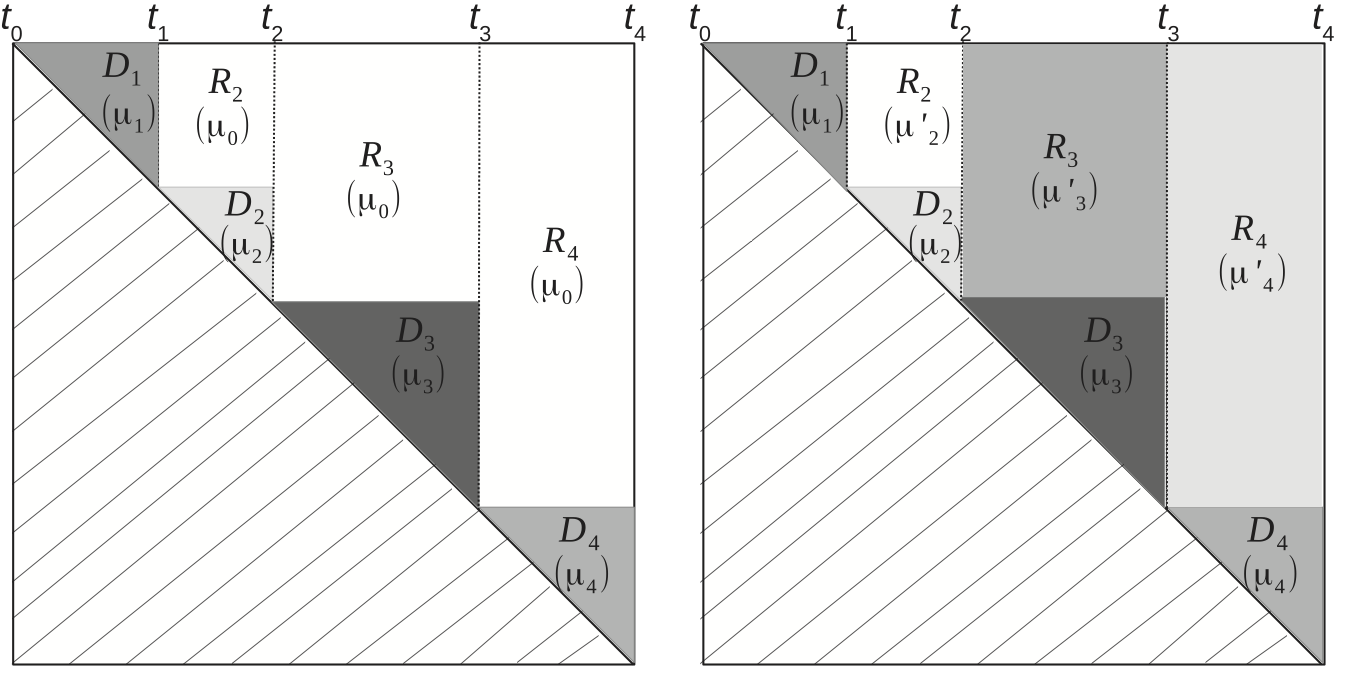
\includegraphics[scale=0.5]{leduc.png}
\end{figure}

\begin{itemize}
\item Partitions into TAD segments by optimizing maximum likelihood
  via dynamic programming
\begin{itemize}
\item Related to 1D and 2D segmentation problems
\end{itemize}
\vspace{0.1cm}
\item Does not allow identificaton of multiscale or
  hierarchical domains
\end{itemize}

\footcitetext{levy2014}

\end{frame}


\begin{frame}
\frametitle{Weaknesses of the existing methods}

\begin{itemize}
\item \textbf{Dixon et al.} : 
\begin{itemize}
\item It is slow and it has many parameters 
\vspace{0.05cm}
\item It is limited to a single scale
\end{itemize}
\vspace{0.1cm}
\item \textbf{Armatus} :
\begin{itemize}
\item Scaling parameter is not linear with respect to avg. domain size
\end{itemize}
\vspace{0.1cm}
\item \textbf{HICseq} :
\begin{itemize}
\item Each segment must belong to a domain
\end{itemize}
\vspace{0.1cm}
\item \textbf{Sefer et al.} :
\begin{itemize}
\item Not scalable to recent high resolution datasets
\end{itemize}
\end{itemize}

\end{frame}


% \begin{frame}
% \frametitle{Weaknesses of the existing methods}

% \begin{itemize}
% \item
% \end{itemize}

% \end{frame}


\begin{frame}
\frametitle{Open Problems}

\begin{itemize}
\item How to find TADs jointly over multiple species?
\vspace{0.1cm}
\item How to find true TAD boundaries efficiently over mixture cell populations?
\end{itemize}

\end{frame}


% \begin{frame}
% \frametitle{Open Problems}

% \begin{itemize}
% \item 
% \vspace{0.1cm}
% \item
% \end{itemize}

% \end{frame}


\begin{frame}
\frametitle{Conclusion}

\begin{itemize}
\item 
\vspace{0.1cm}
\item
\vspace{0.1cm}
\item
\end{itemize}

\end{frame}


\begin{frame}
\frametitle{Acknowledgements}

\vspace{0.8cm}

\begin{itemize}
\item\textcolor{red}{Thanks to Kingsford Group Members}

\vfill

\begin{figure}

\includegraphics[width=1.3cm]{sloan.jpg} 
\hfill

\includegraphics[width=1.3cm]{moorelogo.png} 
\hfill

\includegraphics[width=1.3cm]{nih.png}
\hfill

\includegraphics[width=1.3cm]{nsf.png}
\hfill

\includegraphics[width=1.2cm]{cmulogo.jpeg} 
\hfill

\includegraphics[width=1.0cm]{cpcblogo.jpeg}
\end{figure}
\vfill

\end{itemize}

\end{frame}


\end{document}
